\documentclass[tikz]{standalone}
\usepackage{amsmath,amssymb}
\usepackage{pgfplots,multicol}

\pgfplotsset{compat=1.10}
\usepgfplotslibrary{fillbetween}

\begin{document}



 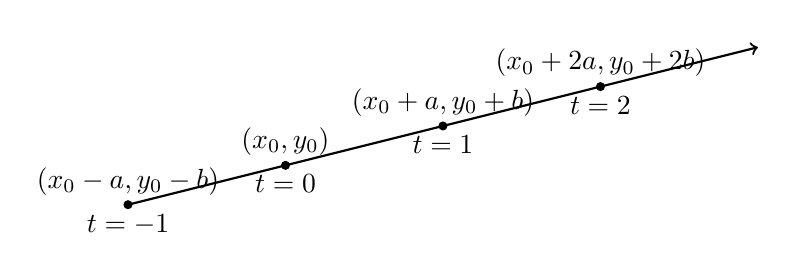
\begin{tikzpicture}[]

%	\foreach \x in {-4,-2,2,4,6}
%	 \draw[-,thick] (\x,0.1) -- (\x,-0.1) node[below] {\x};
%	 
%	 	\foreach \y in {-4,-2,2,4,6}
%	 \draw[-,thick] (0.1,\y) -- (-0.1,\y) node[left] {\y};
	
	
\draw[fill=black] (0,0) circle (0.05cm) node[above] {$(x_0-a,y_0-b)$} node[below]{$t=-1$};
\draw[fill=black] (2,0.5) circle (0.05cm) node[above] {$(x_0,y_0)$} node[below]{$t=0$};
\draw[fill=black] (4,1) circle (0.05cm) node[above] {$(x_0+a,y_0+b)$} node[below]{$t=1$};
\draw[fill=black] (6,1.5) circle (0.05cm) node[above] {$(x_0+2a,y_0+2b)$} node[below]{$t=2$};


\draw[->,thick] (0,0) -- (8,2) node[above] {};

\end{tikzpicture}


	
\end{document}
